% \section*{Midterm 1 Review}

\renewcommand{\arraystretch}{1.25}

\subsection*{16A Review: Circuit Elements}
\begin{center}
    \begin{tabular}[t]{|c|c|p{60px}|p{225px}|}
        \hline
        Type & Drawing & IV Equation & Description \\ \hline
        \begin{minipage}[c]{80px} Voltage Source \end{minipage} &
        \begin{minipage}[c]{50px} 
            \vspace{5px}
            \begin{circuitikz}[american]
                \draw (0, 0) to[V=$V_S$] (0, -2);
            \end{circuitikz}
            \vspace{5px}
        \end{minipage} &
        \begin{minipage}[c]{60px} $V = V_s$ \end{minipage} &
        \begin{minipage}[t]{225px}
            \vspace{-15px}
            The voltage across a voltage source is guaranteed to be $V_S$, regardless of current drawn.
        \end{minipage} \\ \hline
        \begin{minipage}[c]{80px} Current Source \end{minipage} &
        \begin{minipage}[c]{50px} 
            \vspace{5px}
            \begin{circuitikz}[american]
                \draw (0, -2) to[isource, l=$I_S$] (0, 0);
            \end{circuitikz}
            \vspace{5px}
        \end{minipage} &
        \begin{minipage}[c]{60px} $I = I_s$ \end{minipage} &
        \begin{minipage}[t]{225px}
            \vspace{-15px}
            The current produced by a current source is guaranteed to be $I_S$, regardless of the voltage across it.
        \end{minipage} \\ \hline
        \begin{minipage}[c]{80px} Resistor \end{minipage} &
        \begin{minipage}[c]{50px} 
            \vspace{5px}
            \begin{circuitikz}[american]
                \draw (0, 0) to[R=$R$, v=$V\,\,$, i=$I$] (0, -2);
            \end{circuitikz}
            \vspace{5px}
        \end{minipage} &
        \begin{minipage}[c]{60px} \textbf{Ohm's Law}: \\ $V = IR$ \end{minipage} &
        \begin{minipage}[t]{225px}
            \vspace{-15px}
            A resistor causes a voltage drop proportional to the current flowing across it.
        \end{minipage} \\ \hline
        \begin{minipage}[c]{80px} Capacitor \end{minipage} &
        \begin{minipage}[c]{50px} 
            \vspace{5px}
            \begin{circuitikz}[american]
                \draw (0, 0) to[C=$C$, v=$V\,\,$, i=$I$] (0, -2);
            \end{circuitikz}
            \vspace{5px}
        \end{minipage} &
        \begin{minipage}[c]{60px} $Q = CV$ \\ 
        
        $I = C\frac{dV}{dt}$ \end{minipage} &
        \begin{minipage}[t]{225px}
            \vspace{-30px}
            A capacitor stores an amount of charge proportional to the voltage across it. An uncharged capacitor connected to a voltage source via a resistor will \textbf{charge up}, and a charged capacitor connected to ground via a resistor will \textbf{discharge}.
        \end{minipage} \vspace{2px} \\ \hline
    \end{tabular} 
\end{center}

\subsection*{16A Review: Equivalent Resistance and Capacitance}

\textbf{Resistors in Series}:
\begin{center}
    \begin{circuitikz}[american]
        \draw (0, 0) to[R=$R$, *-] (2, 0)
        (2, 0) to[R=$R$] (4, 0)
        (4, 0) to[R=$R$, -*] (6, 0);
    \end{circuitikz}
    \begin{align*}
        R_{eq} = \sum_i R_i.
    \end{align*}
\end{center}
When resistors are in \textbf{series} (resistors that have the \textit{same current through them}), their resistances \textbf{add}. For instance, the circuit above can be condensed to one resistor of value $3R$. \\
\newpage
\textbf{Resistors in Parallel}:
\begin{center}
    \begin{circuitikz}[american]
        \draw (0, 0) to[R=$R$] (0, -2)
        (0, 0) to[short] (4, 0)
        (0, -2) to[short] (4, -2)
        (2, 0) to[R=$R$] (2, -2)
        (4, 0) to[R=$R$] (4, -2);
    \end{circuitikz}
    \begin{align*}
        1/R_{eq} = \sum_i 1/R_i.
    \end{align*}
\end{center}

When resistors are in \textbf{parallel} (they have the \textit{same voltage across them}, i.e. share two nodes), the \textbf{inverses of their resistances add}.
For instance, the circuit above can condensed to one resistor of value $R/3$.  \\

\textbf{Capacitors in Series}:
\begin{center}
    \begin{circuitikz}[american]
        \draw (0, 0) to[C=$C$, *-] (2, 0)
        (2, 0) to[C=$C$] (4, 0)
        (4, 0) to[C=$C$, -*] (6, 0);
    \end{circuitikz}
    \begin{align*}
        1/C_{eq} = \sum_i 1/C_i.
    \end{align*}
\end{center}

For capacitors in series, the \textbf{inverses of their capacitances add} (just like resistors in parallel). \\

\textbf{Capacitors in Parallel}:
\begin{center}
    \begin{circuitikz}[american]
        \draw (0, 0) to[C=$C$] (0, -2)
        (0, 0) to[short] (4, 0)
        (0, -2) to[short] (4, -2)
        (2, 0) to[C=$C$] (2, -2)
        (4, 0) to[C=$C$] (4, -2);
    \end{circuitikz}
    \begin{align*}
        C_{eq} = \sum_i C_i.
    \end{align*}
\end{center}

For capacitors in parallel, their \textbf{capacitances add} (just like resistors in series).

\subsection*{16A Review: Passive Sign Convention}
We use \textbf{passive sign convention} to define currents and voltages relative to each other in or circuit analysis.
\begin{center}
    \begin{circuitikz}[american]
        \draw (0, 0) to[R=$R$, i=$i_R$, v=$v_R$] (3, 0);
    \end{circuitikz}
\end{center}
\begin{align*}
    v_R = v_+ - v_-
\end{align*}
We define the voltage across an element such that current flows from the \textbf{positive end of the voltage to the negative end}. The motivation for this is to label voltages and currents such that elements that consume power always have a \textit{positive power value} ($p = iv$).

\subsection*{16A Review: KCL and KVL}
\textbf{KCL (Kirchhoff's Current Law)}: The sum of all \textit{currents entering a node is equal to the sum of all currents leaving a node}.

\begin{center}
    \begin{circuitikz}[american]
        \draw (0, 0) to[R=$R_1$, i^<=$i_1$, -*] (3, 0) node[above] {$V_1$}
        (3, 0) to[R=$R_2$, i>^=$i_2$] (3, -2.5)
        (3, 0) to[R=$R_3$, i>^=$i_3$] (6, 0);
    \end{circuitikz}
\end{center}
In the above circuit, the KCL equation for $V_1$ is
\begin{align*}
    i_1 + i_2 + i_3 = 0.
\end{align*}

\textbf{KVL (Kirchhoff's Voltage Law)}: The sum of \textit{voltages in any closed loop is 0}. When applying KVL:
\begin{enumerate}
    \item Pick a loop, a node to start at, and a direction (clockwise or counterclockwise).
    \item Go through the loop in the direction you chose, filling out the sum of voltage in the loop ($\sum V$). \textbf{Add voltages} if you go from the \textit{negative end to the positive end}, and \textbf{subtract voltages} if you go from the \textit{positive end to the negative end}.
    \item Set the sum equal to 0.
\end{enumerate}

\begin{center}
    \begin{circuitikz}[american]
        \draw (0, 0) to[R, l_=$R_1$, v^<=$v_1$] (2.5, 0)
        (2.5, 0) to[R, l_=$R_2$, v^>=$v_2$] (2.5, -2.5)
        (2.5, -2.5) to[R, l_=$R_3$, v^>=$v_3$] (0, -2.5)
        (0, -2.5) to[R, l_=$R_4$, v^<=$v_4$] (0, 0);
    \end{circuitikz}
\end{center}
For instance, at the circuit above, let us choose to go clockwise starting at the negative end of $R_1$. We are going from the negative end to positive end of $R_1$ and $R_4$, so we \textbf{add} $v_1$ and $v_4$ to our sum of voltages. We are going from the positive end to the negative end of $R_2$ and $R_3$, so we \textbf{subtract} $v_2$ and $v_3$. Overall, we get

\begin{align*}
    v_1 - v_2 - v_3 + v_4 = 0.
\end{align*}

\subsection*{Voltage and Current Dividers}
Two common circuit configuration that you may see are \textbf{voltage dividers} and \textbf{current dividers}. 
\newpage
\textbf{Voltage Dividers}:
\begin{center}
    \begin{circuitikz}
        \draw (0, 0) to[V=$V_S$] (0, -3)
        (0, 0) to[R=$R_1$] (3, 0) 
        (3, 0) to[R, l_=$R_2$, v^=$V_{out}$] (3, -3)
        (0, -3) to[short] (3, -3);
    \end{circuitikz}
\end{center}
Using KCL, KVL, and Ohm's Law, we find that the voltage across $R_2$ is
\begin{align*}
    V_{out} = \frac{R_2}{R_1 + R_2} V_S.
\end{align*}

\textbf{Current Divider}:
\begin{center}
    \begin{circuitikz}
        \draw (0, 0) to[V=$V_S$, i<_=$i_S$] (0, -2)
        (0, 0) to[short] (4, 0)
        (0, -2) to[short] (4, -2)
        (2, 0) to[R=$R_1$, i>_=$i_1$] (2, -2) 
        (4, 0) to[R=$R_2$, i>_=$i_2$] (4, -2)
        (0, -2) to[short] (4, -2);
    \end{circuitikz}
\end{center}
A current divider is similar to a voltage divider, in that we can write the current going through $R_1$ as
\begin{align*}
    i_1 = \frac{i_2}{i_1 + i_2} i_S.
\end{align*}

\subsection*{Nodal Analysis}
Nodal analysis uses a combination of KCL, KVL and element IV relationships to solve more complicated circuits that cannot be reduced to voltage or current dividers.

\textbf{Procedure}:
\begin{enumerate}
    \item Label a \textbf{ground} in your circuit. This node is arbitrarily chosen to have zero potential.
    \item Label the potentials of nodes where you know the potential. These are typically nodes at the positive end of a voltage source.
    \item Label the other nodes with a variable ($V_1$, $V_2$, etc.) representing their potential.
    \item For each unknown node, label the currents leaving that node and write out a \textbf{KCL} equation.
    \item Use \textbf{element current-voltage relationships} to write the currents in your KCL equation in terms of potentials in your circuit.
    \item Now, you have equations to solve for the unknown voltages in your circuit!
\end{enumerate}

\textit{Note: Any two points in the circuit that are connected \textbf{only by a wire} are in the same node. The entire node is at the same potential.}

\subsection*{Superposition}
Superposition is a tool that you can use to solve circuits with \textit{multiple voltage or current sources}. 

\textbf{Procedure}:
\begin{enumerate}
    \item For each \textit{independent source}:
    \begin{enumerate}
        \item \textbf{Null all of the other sources}. This means \textit{replacing voltage sources with a wire} and \textit{replacing current sources with an open circuit}. Note that nulling a voltage source sets the voltage across it to 0, and nulling a current source sets the current through it to 0.
        \item Solve for the voltage or current in question. We will call that the solution to this \textit{sub-problem}.
    \end{enumerate}
    \item Your final voltage or current is the sum of your results from each sub-problem!
\end{enumerate}

\subsection*{Op-Amps}
\textbf{Ideal Op-Amps}: 
We can model an op-amp using a dependent voltage source and resistors:
\begin{center}
    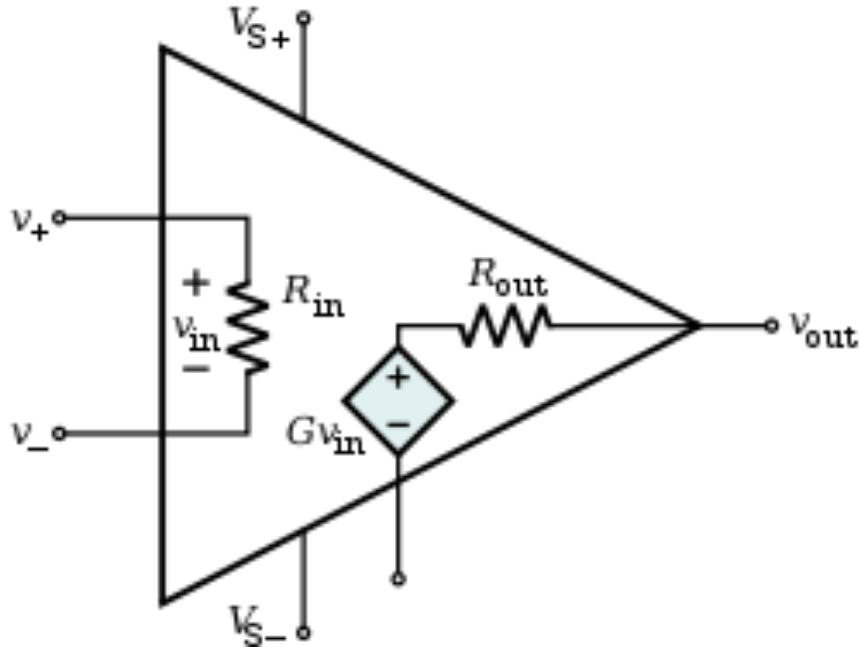
\includegraphics[width=0.5\textwidth]{opamp_model.png}
\end{center}
We care about \textbf{ideal op-amps}, where:
\begin{enumerate}
    \item $R_{in} = \infty$
    \item $G = \infty$
    \item $R_{out} = 0$
\end{enumerate}
\textit{Note: the maximum $V_{out}$ can be is $V_{S+}$, the positive power supply, and the minimum $V_{out}$ can be is $V_{S-}$. If $Gv_{in}$ isn't in those bounds, we say that the output \textbf{rails} to $V_{S+}$ or $V_{S-}$.}

From these properties of ideal op-amps, we can derive the \textbf{op-amp golden rules}:
\begin{enumerate}
    \item For all ideal op-amps, \textbf{no current flows into the + or - terminal}.
    \item For op-amps in \textbf{negative feedback}, $v_+ = v_-$
\end{enumerate}
\textit{Note: \textbf{Negative feedback} typically occurs when the output feeds back into the negative terminal.}

\textit{To see why, imagine the output voltage increases slightly. This causes $v_-$ to increase slightly, which in turn decreases $V_{out} = G(v_+ - v_-)$.} \\

\textbf{Common Op-Amp Configurations - Buffer}: 
A buffer guarantees that $V_{out}$ is equal to $V_{in}$.

We often use buffers to prevent \textbf{loading}, a phenomenon where \textit{attaching a load resistance (or another element that draws current) to the output of a circuit changes its output voltage}. If loading may occur, \textit{place a buffer between the output voltage of your circuit and the load}.
\begin{center}
    \begin{circuitikz}[american]
        \draw (0, 0) node[op amp, yscale=-1] (opamp) {}
        (opamp.+) to[short, -o] (-1.3, 0.5) node[label={left:$V_{in}$}] {}
        (opamp.-) to[short] (-1.2, -1.5) node[] (bottom) {}
        (bottom) to[short] (1.3, -1.5)
        (1.3, -1.5) to[short] (1.3, 0)
        (opamp.out) to[short, -o] (1.5, 0) node[label={right:$V_{out}$}] {};
    \end{circuitikz}
\end{center}
\begin{align*}
    V_{out} = V_{in}.
\end{align*}

\textbf{Common Op-Amp Configurations - Inverting Amplifier}:
An inverting amplifier scales the input voltage by a negative number.
\begin{center}
    \begin{circuitikz}[american]
        \draw (0, 0) node[op amp] (opamp) {}
        (opamp.-) to[short] (-1.2, 1.5) node[] (top) {}
        (top) to[R=$R_2$] (1.3, 1.5)
        (1.3, 1.5) to[short] (1.3, 0)
        (opamp.out) to[short, -o] (1.5, 0) node[label={right:$V_{out}$}] {}
        (opamp.-) to[R, l_=$R_1$, -o] (-2.7, 0.5) node[label={left:$V_{in}$}] {}
        (opamp.+) to[short] (-1.3, -0.5) node[ground] {};
    \end{circuitikz}
\end{center}
\begin{align*}
    V_{out} = -V_{in} \frac{R_2}{R_1}.
\end{align*}

\textbf{Common Op-Amp Configurations - Non-Inverting Amplifier}:
A non-inverting amplifier scales the input voltage by a positive number.
\begin{center}
    \begin{circuitikz}[american]
        \draw (0, 0) node[op amp, yscale=-1] (opamp) {}
        (opamp.+) to[short, -o] (-1.3, 0.5) node[label={left:$V_{in}$}] {}
        (opamp.-) to[short] (-1.2, -1.5) node[] (bottom) {}
        (-3.3, -1.5) node[ground] {} to[R=$R_1$] (bottom)
        (bottom) to[R=$R_2$] (1.3, -1.5)
        (1.3, -1.5) to[short] (1.3, 0)
        (opamp.out) to[short, -o] (1.5, 0) node[label={right:$V_{out}$}] {};
    \end{circuitikz}
\end{center}
\begin{align*}
    V_{out} = V_{in} \cdot (1 + R_2 / R_1).
\end{align*}

\subsection*{MOSFET Behavior and Models}

\begin{center} 
\begin{tabular}[t]{|c|c|p{60px}|p{275px}|}
\hline
Type & Drawing & Switch Closed & Behavior \\ \hline
 \begin{minipage}[c]{30px} PMOS \end{minipage} & \begin{minipage}[c]{50px} \begin{circuitikz}[american] 
\draw (0, 0) node[pmos, emptycircle] (nmos) {};
\draw (nmos.G) node[left]{$G$};
\draw (nmos.S) node[left]{$S$};
\draw (nmos.D) node[left]{$D$};
\end{circuitikz}
\end{minipage} & 
\begin{minipage}[c]{60px} $V_{GS} \leq -|V_{tp}|$ \end{minipage} &
\begin{minipage}[t]{275px}
\vspace{-15px}
Closed switch when gate voltage $V_G$ is at least $|V_{tp}|$ below source voltage $V_S$ (gate voltage is low). Open switch otherwise.
\end{minipage} \\ \hline
\begin{minipage}[c]{30px} NMOS \end{minipage} & 
\begin{minipage}[c]{50px}
\begin{circuitikz}[american] 
\draw (0, 0) node[nmos] (nmos) {};
\draw (nmos.G) node[left]{$G$};
\draw (nmos.S) node[left]{$S$};
\draw (nmos.D) node[left]{$D$};
\end{circuitikz}
\end{minipage} & 

\begin{minipage}[c]{60px} $V_{GS} \geq |V_{tn}|$ \end{minipage} &

\begin{minipage}[t]{275px}
\vspace{-15px}
Closed switch when gate voltage $V_G$ is at least $V_{tn}$ above source voltage $V_S$ (gate voltage is high). Open switch otherwise.
\end{minipage} \\ \hline
\end{tabular} \end{center}

\begin{center} \begin{tabular}{|c|c|c|c|}
\hline
Type & (Voltage-Controlled) Switch & Resistor-Switch & Resistor-Capacitor-Switch \\ \hline
\begin{minipage}[c]{30px} \vspace{-110px} PMOS \end{minipage}
 & \begin{circuitikz}[scale=0.9]
			\draw (0, -2) node[label=left:$D$] {}
			to[switch, l_= $V_{GS} \leq -|V_{tp}|$, *-] (0,2)
			to[short, -*] ++(0, 0.2)
            node[label=right:$S$] {};;
			\draw (0, 2) -- (-1, 2) to [short, -o] (-1, 2);;
            \draw (-2, 0) to [short, -*] (-2, 0)
                          to [short, -o] (-1, 0) node[label=below:$G$] {}
                          to [open, v^=$V_{GS}$] ++(0, 2);;
			% to[short, -*] ++(0, -2) node[label=left:$G$] {};;
            % \draw (-1, -2) node[label=left:$G$] {};;
			\draw (0, -1.75) to [short, -*, l=$V_{out}$] ++(1,0);;
		\end{circuitikz} & 
        \begin{circuitikz}[scale=0.9]
			\draw (0, -2) node[label=left:$D$] {}
			to[switch,l_= $V_{GS} \leq -|V_{tp}|$, *-] (0,0)
			to[R, l_=$R_{on, P}$, i<=$I_D$] ++(0, 2)
			to[short, -*] ++(0, 0.2) node[label=right:$S$] {};;
            \draw (0, 2) -- (-1, 2) to [short, -o] (-1, 2);;
            \draw (-2, 0) to [short, -*] (-2, 0)
                          to [short, -o] (-1, 0) node[label=below:$G$] {}
                          to [open, v^=$V_{GS}$] ++(0, 2);;

			% \draw (0, 2) -- (-1, 2)
			% to[short, -*] ++(0, -2) node[label=left:$G$] {};;
			\draw (0, -1.75) to [short, -*, l=$V_{out}$] ++(1,0);;
		\end{circuitikz} &
        \begin{circuitikz}[scale=0.9]
			\draw (0, -2) node[label=left:$D$] {}
			to[switch,l_= $V_{GS} \leq -|V_{tp}|$, *-] (0,0)
			to[R, l_=$R_{on, P}$, i<=$I_D$] ++(0, 2)
			to[short, -*] ++(0, 0.2)
            node[label=right:$S$] {};;
			\draw (0, 2) -- (-2, 2);;
			\draw (-2, 0) to[short, -*] ++(0, 0) node[label=left:$G$] {} to[C, l_=$C_{GS}$, v^=$V_{GS}$] ++(0, 2);;
			\draw (0, -1.75) to [short, -*, l=$V_{out}$] ++(1,0);;
		\end{circuitikz} \\ \hline

\begin{minipage}[c]{30px} \vspace{-110px} NMOS \end{minipage}
 & \begin{circuitikz}[scale=0.9]
            \draw (0,-2)
            to[switch,l_= $V_{GS} \geq V_{tn}$]
            (0,2) to[short, -*] ++(0,0)
            node[label=left:$D$] {};;
            % \draw (0,-2) -- (-1,-2)
            % to[short, -*] ++(0,2) node[label=left:$G$] {};;
            \draw (0, -2) -- (-1, -2) to [short, -o] (-1, -2);;
            \draw (-2, 0) to [short, -*] (-2, 0)
                          to [short, -o] (-1, 0) node[label=above:$G$] {}
                          to [open, v=$V_{GS}$] ++(0, -2);;

            \draw (0,1.75) to [short,-*,l=$V_{out}$] ++ (1,0);;
            \draw (0, -2) to [short, -*] ++(0, -0.2) node[label=right:$S$] {};;
        \end{circuitikz} &
        \begin{circuitikz}[scale=0.9]
            \draw (0,-2)
            to[switch,l_= $V_{GS} \geq V_{tn}$]
            (0,0) to[R,-*,l=$R_{on, N}$,i<=$I_D$] ++(0,2)
            node[label=left:$D$] {};;
            % \draw (0,-2) -- (-1,-2)
            % to[short, -*] ++(0,2) node[label=left:$G$] {};;
            \draw (0, -2) -- (-1, -2) to [short, -o] (-1, -2);;
            \draw (-2, 0) to [short, -*] (-2, 0)
                          to [short, -o] (-1, 0) node[label=above:$G$] {}
                          to [open, v=$V_{GS}$] ++(0, -2);;

            \draw (0,1.75) to [short,-*,l=$V_{out}$] ++ (1,0);;
            \draw (0, -2) to [short, -*] ++(0, -0.2) node[label=right:$S$] {};;
        \end{circuitikz} & 
        \begin{circuitikz}[scale=0.9]
            \draw (0,-2)
            to[switch,l_= $V_{GS} \geq V_{tn}$]
            (0,0) to[R,-*,l=$R_{on, N}$,i<=$I_D$] ++(0,2)
            node[label=left:$D$] {};;
            \draw (0,-2) -- (-2,-2);;
            \draw (-2, 0) to [short, -*] (-2, 0) node[label=left:$G$] {} to[C,l=$C_{GS}$,v=$V_{GS}$] ++(0,-2);;
            \draw (0,1.75) to [short,-*,l=$V_{out}$] ++(1,0);;
            \draw (0, -2) to [short, -*] ++(0, -0.2) node[label=right:$S$] {};;
        \end{circuitikz} \\ \hline
\end{tabular} 
\end{center}

\newpage
\subsection*{CMOS Circuits and Logic Gates}
We can use MOSFETS to perform logic functions by implementing \textbf{pull-up} and \textbf{pull-down} networks. Logic gates typically consist of:
\begin{enumerate}
    \item \textit{A pull-up network of \textbf{PMOS transistors} between $V_{DD}$ and the output}.
    \begin{enumerate}
        \item This network should provide a path from $V_{DD}$ to the output when the logic expression is \textbf{true}.
        \item Remember, the gates on the PMOS transistors will be \textbf{closed} when the corresponding input voltage is \textbf{low} ($V_{GS} = V_{in} - V_{DD}$, which passes the threshold when $V_{in}$ is low, or $0$).
    \end{enumerate}
    \item A \textit{pull-down network of \textbf{NMOS transistors} between the output and ground}. 
    \begin{enumerate}
        \item This network should provide a path from the output to ground if the expression is \textbf{false}.
        \item Remember, the gates on the NMOS transistors will be \textbf{closed} when the corresponding input voltage is \textbf{high} ($V_{GS} = V_{in} - 0$, which is greater than the threshold when $V_{in}$ is high, or $V_{DD}$).
    \end{enumerate}
\end{enumerate}

\textbf{Example: CMOS Inverter}
\begin{center}
    \begin{circuitikz}[american]
    \draw (0,-0.75) node[pmos, emptycircle] (pmos) {} 
        (0, 0) node[vdd, above] {$V_{DD}$} to[short] (pmos.source)
        (pmos.drain) to[short] (0, -2)
        (0, -2) to[short, -*] (0.5, -2) node[above] {$V_{out}$}
        (0, -3) node[nmos] (nmos) {}
        (0, -2) to[short] (nmos.drain) 
        (nmos.source) to[short] (0, -4) node[ground] {}
        (-1.25, -0.75) node[left] {$V_{in}$} to[short, *-] (pmos.gate)
        (-1.25, -3) node[left] {$V_{in}$} to[short, *-] (nmos.gate);
    \end{circuitikz}
\end{center}

\begin{enumerate}
    \item When the input is high ($V_{in} = V_{DD}$), the PMOS transistor is an open circuit, and the NMOS switch is closed, creating a path between the output and ground. $V_{out} = 0$.
    \item When the input is low ($V_{in} = 0$), the PMOS switch is closed, creating a path between $V_{DD}$ and the output. The NMOS transistor is an open circuit. $V_{out} = V_{DD}$.
\end{enumerate}

\newpage
\textbf{Example: NAND Gate}
\begin{center}
    \begin{circuitikz}
        \draw (6,5) node[pmos, emptycircle](pm){} ;
        \draw (3.5,5) node[pmos, emptycircle](pm1){} ;
        \draw (6,1) node[nmos](nm){} ;
        \draw (6,3) node[nmos](nm1){} ;
        \draw (pm1.gate) to [short, -*](1,5) node[left]{$V_{A}$};
        \draw (nm1.gate) to [short, -*](1, 3) node[left]{$V_{B}$};
        \draw [short, *-] (2,5) to (2,1);
        \draw [short] (2,1) to (nm.gate);
        \draw (pm.source) to [short] (6,6) node[vdd, above]{$V_{DD}$};
        \draw (pm1.source) to [short] (3.5,6) node[vdd, above]{$V_{DD}$};
        \draw (pm.drain) to (nm1.drain);
        \draw (nm1.source) to (nm.drain);
        \draw [short, *-] (4.5,3) to (4.5,5);
        \draw [short] (4.5,5) to (pm.gate);
        \draw (pm1.drain) to (3.5,4) to [short] (6,4) 
        (6, 4) to[short, -*] (6.5, 4) node[right]{$V_o$};
        \draw (nm.source) to (6,0) node[ground]{};
    \end{circuitikz}
\end{center}

\begin{enumerate}
    \item When both $V_A$ and $V_B$ are high, both PMOS transistors are open circuits, and both NMOS switches are closed, providing a path to ground. $V_{out} = 0$.
    \item When either $V_A$ or $V_B$ are low, at least one PMOS switch is closed, so there is a path from $V_{DD}$ to the output. At least one NMOS switch is open, so the output isn't connected to ground. $V_{out} = V_{DD}$.
\end{enumerate}

\textbf{Example: NOR Gate}

\begin{center}
    \begin{circuitikz}
        \draw (6,5) node[pmos, emptycircle](pm){} ;
        \draw (6,3) node[pmos, emptycircle](nm){} ;
        \draw (6,1) node[nmos]
        (n){} ;
        \draw (3.5,1) node[nmos]
        (nq){} ;
        \draw (pm.gate) to [short, -*](1,5) node[left]{$V_{in, 1}$};
        \draw [short, *-] (2,5) to (2,1);
        \draw [short] (2,1) to (nq.gate);
        \draw (nq.drain) to [short](3.5,2) to [short, -*](6,2) ;
        \draw (pm.source) to [short] (6,6) node[above, vdd]{$V_{DD}$};
        \draw (pm.drain) to (nm.source);
        \draw (nm.gate) to [short, -*](4, 3) to [short](4,1)  to (n.gate);
        \draw [short](4,3) to [short, -*](1, 3) node[left]{$V_{in, 2}$};
        \draw (6,2) to [short, -*] (7,2) node[right]{$V_{o}$};
        \draw (n.drain) to (nm.drain);
        \draw (n.source) to [short] (6, -1) to (3.5, -1) to (nq.source);
        \draw [short] (4.75, -1) to (4.75,-1) node[ground]{};
    \end{circuitikz}
\end{center}

\begin{enumerate}
    \item When either $V_A$ and $V_B$ are high, at least one PMOS switch is open, and at least one NMOS switch is closed, providing a path to ground. $V_{out} = 0$.
    \item When both $V_A$ or $V_B$ are low, at both PMOS switches are closed, so there is a path from $V_{DD}$ to the output. Both NMOS switches are open, so the output isn't connected to ground. $V_{out} = V_{DD}$.
\end{enumerate}

\subsection*{Power}

\textbf{Power} is the rate at which energy is produced or consumed.
\begin{align*}
    P = \frac{dE}{dt} = IV. \\
    \Delta E = \int_{t_A}^{t_B} P(t) \, dt.
\end{align*}
\begin{enumerate}
    \item Resistors \textbf{dissipate} power as current passes through them.
    \begin{align*}
        P = IV = I^2R = V^2/R.
    \end{align*}
    The power value of a resistor should be \textbf{positive}, indicating energy consumed.

    \item Capacitors \textbf{store energy} when charging, and \textbf{release energy} when discharging.
    \begin{align*}
        \Delta E_{\text{charging}} = \frac{1}{2} CV_s^2. \\
        \Delta E_{\text{discharging}} = -\frac{1}{2} CV_s^2.
    \end{align*}

    \item Typically (but not always), voltage and current sources \textbf{supply power}. When using $P = IV$ to calculate the power of a source, be careful about using passive sign convention! A source supplying power to the circuit (which is most cases you'll see) should have a \textbf{negative} power.
\end{enumerate}

\subsection*{Transistor Power Consumption}

\textbf{CMOS networks} do not consume power in steady state, but they do consume power when switching.

Consider a CMOS inverter with a capacitor connected to the output. You can think of this as the \textit{gate capacitance} of another transistor (in real life, the output of one CMOS network is typically the input to another CMOS network).
\begin{center}
    \begin{circuitikz}[american]
        \draw (0,-0.75) node[pmos, emptycircle] (pmos) {} 
        (0, 0) node[vdd, above] {$V_{DD}$} to[short] (pmos.source)
        (pmos.drain) to[short] (0, -2)
        (0, -2) to[short] (1.5, -2) node[above] {$V_{out}$}
        (1.5, -2) to[C=$C$] (1.5, -4) node[ground] {}
        (0, -3) node[nmos] (nmos) {}
        (0, -2) to[short] (nmos.drain) 
        (nmos.source) to[short] (0, -4) node[ground] {}
        (-1.25, -0.75) node[left] {$V_{in}$} to[short, *-] (pmos.gate)
        (-1.25, -3) node[left] {$V_{in}$} to[short, *-] (nmos.gate);
    \end{circuitikz}
\end{center}
When the output switches from low to high, we can redraw the above circuit as follows:
\begin{center}
    \begin{circuitikz}[american]
        \draw (0, 0) to[V=$V_{DD}$] (0, -2) node[ground] {}
        (0, 0) to[R=$R_{on}$, -*] (3, 0) node[right] {$V_{out}$}
        (3, 0) to[C=$C_{GS}$] (3, -2) node[ground] {};
    \end{circuitikz}
\end{center}
If we assume that the output had been low for a long time before switching, the capacitor starts out \textbf{discharged}, and \textbf{charges up} to $V_{DD}$.

The capacitor stores energy while charging, the resistor dissipates energy, and the voltage source supplies energy:
\begin{enumerate}
    \item $\Delta E_C = \frac{1}{2} CV_{DD}^2$.
    \item $\Delta E_R = \frac{1}{2} CV_{DD}^2$. This can be found by solving for the power consumption of the resistor with respect to time, and then integrating from $t = 0$ to $t=\infty$. Finding the power value involves solving a differential equation, which is not in scope for the quest.
    \item $\Delta E_{V_{DD}} = -(\Delta E_C + \Delta E_R) = CV_{DD}^2$. 
\end{enumerate}

When the output switches from low to high, the network can be represented as the following circuit:
\begin{center}
    \begin{circuitikz}[american]
        \draw (0, 0) to[short] (0, -2) node[ground] {}
        (0, 0) to[R=$R_{on}$, -*] (3, 0) node[right] {$V_{out}$}
        (3, 0) to[C=$C_{GS}$] (3, -2) node[ground] {};
    \end{circuitikz}
\end{center}

The capacitor releases energy and the resistor dissipates energy:
\begin{enumerate}
    \item $\Delta E_C = -\frac{1}{2} CV_{DD}^2$.
    \item $\Delta E_R = \frac{1}{2} CV_{DD}^2$.
\end{enumerate}
\newpage
On the other hand, \textbf{NMOS and PMOS networks} consume energy while in steady state.

For instance, consider an NMOS inverter:
\begin{center}
    \begin{circuitikz}[american]
        \draw (0, 0) node[vdd, above] {$V_{DD}$} to[R=$R$] (0, -1.5)
        (0, -1.5) to[short, -*] (0.5, -1.5) node[right] {$V_{out}$}
        (0, -2.5) node[nmos] (nmos) {}
        (0, -1.5) to[short] (nmos.drain) 
        (nmos.source) to[short] (0, -3) node[ground] {}
        (-1.25, -2.5) node[left] {$V_{in}$} to[short, *-] (nmos.gate);
    \end{circuitikz}
\end{center}
When the output is high, the NMOS switch is open, so there is no path for current to flow through $R$. 

However, when the \textbf{output is low}, the NMOS switch is closed and current can flow from $V_{DD}$ to ground:

\begin{center}
    \begin{circuitikz}[american]
        \draw (0, 0) node[vdd, above] {$V_{DD}$} to[R=$R$] (0, -1.5)
        (0, -1.5) to[short, -*] (0.5, -1.5) node[right] {$V_{out}$}
        (0, -1.5) to[R=$R_{on}$] (0, -3) node[ground] {};
    \end{circuitikz}
\end{center}
The power dissipated by the resistors is
\begin{align*}
    P = IV = \frac{V_{DD}^2}{R + R_{on}}.
\end{align*}

A \textbf{PMOS inverter} (pictured below) consumes the same amount of power as an NMOS inverter, but when the output is \textbf{high} instead of low (the switch on the PMOS is closed, so current flows from $V_{DD}$ to ground).

\begin{center}
    \begin{circuitikz}[american]
        \draw (0,-0.5) node[pmos, emptycircle] (pmos) {} 
        (0, 0) node[vdd, above] {$V_{DD}$} to[short] (pmos.source)
        (pmos.drain) to[short] (0, -1.5)
        (0, -1.5) to[short, -*] (0.5, -1.5) node[above] {$V_{out}$}
        (0, -1.5) to[R=$R$] (0, -3) node[ground] {}
        (-1.25, -0.5) node[left] {$V_{in}$} to[short, *-] (pmos.gate);
    \end{circuitikz}
\end{center}